%----------------------------------------------------------------------------------------
%	PACKAGES AND OTHER DOCUMENT CONFIGURATIONS
%----------------------------------------------------------------------------------------

\documentclass[11pt,a4paper]{article}

\usepackage[a4paper,margin=2cm]{geometry}

\usepackage{fancyhdr} % Required for custom headers
\usepackage{lastpage} % Required to determine the last page for the footer
\usepackage{extramarks} % Required for headers and footers
\usepackage[usenames,dvipsnames]{color} % Required for custom colors
\usepackage{graphicx} % Required to insert images
\usepackage{listings} % Required for insertion of code
\usepackage{courier} % Required for the courier font
\usepackage{lipsum} % Used for inserting dummy 'Lorem ipsum' text into the template
\usepackage{parskip}
% Margins
\topmargin=-0.45in
%\evensidemargin=0in
%\oddsidemargin=0in
%\textwidth=6.5in
%\textheight=9.0in
\headsep=0.25in
\definecolor{mygreen}{rgb}{0,0.51, 0}
%\linespread{1.1} % Line spacing

% Set up the header and footer
\pagestyle{fancy}
\chead{} % Top left header
\lhead{\hmwkClass\  \hmwkTitle} % Top center head
\rhead{} % Top right header
\lfoot{\lastxmark} % Bottom left footer
\cfoot{} % Bottom center footer
\rfoot{Page\ \thepage\ of\ \protect\pageref{LastPage}} % Bottom right footer
\renewcommand\headrulewidth{0.4pt} % Size of the header rule
\renewcommand\footrulewidth{0.4pt} % Size of the footer rule

\setlength\parindent{0pt} % Removes all indentation from paragraphs

%----------------------------------------------------------------------------------------
%	CODE INCLUSION CONFIGURATION
%----------------------------------------------------------------------------------------

% \definecolor{MyDarkGreen}{rgb}{0.0,0.4,0.0} % This is the color used for comments
\lstloadlanguages{C} % Load C syntax for listings, for a list of other languages supported see: ftp://ftp.tex.ac.uk/tex-archive/macros/latex/contrib/listings/listings.pdf
\lstset{commentstyle=\color{mygreen},basicstyle=\ttfamily\scriptsize,language=C,frame=single,keywordstyle=[1]\color{Blue}\bf} % Use C in this example      



\newcommand{\csnippet}[2]{
\begin{itemize}
\item[]\lstinputlisting[caption=#2,label=#1]{#1.c}
\end{itemize}
}

%----------------------------------------------------------------------------------------
%	DOCUMENT STRUCTURE COMMANDS
%----------------------------------------------------------------------------------------

% Header and footer for when a page split occurs within a problem environment
\newcommand{\enterProblemHeader}[1]{
\nobreak\extramarks{#1}{#1 continued on next page\ldots}\nobreak
\nobreak\extramarks{#1 (continued)}{#1 continued on next page\ldots}\nobreak
}

% Header and footer for when a page split occurs between problem environments
\newcommand{\exitProblemHeader}[1]{
\nobreak\extramarks{#1 (continued)}{#1 continued on next page\ldots}\nobreak
\nobreak\extramarks{#1}{}\nobreak
}

\setcounter{secnumdepth}{0} % Removes default section numbers
\newcounter{homeworkProblemCounter} % Creates a counter to keep track of the number of problems

\newcommand{\homeworkProblemName}{}
\newenvironment{homeworkProblem}[1][Problem \arabic{homeworkProblemCounter}]{ % Makes a new environment called homeworkProblem which takes 1 argument (custom name) but the default is "Problem #"
\stepcounter{homeworkProblemCounter} % Increase counter for number of problems
\renewcommand{\homeworkProblemName}{#1} % Assign \homeworkProblemName the name of the problem
\section{\homeworkProblemName} % Make a section in the document with the custom problem count
\enterProblemHeader{\homeworkProblemName} % Header and footer within the environment
}{
\exitProblemHeader{\homeworkProblemName} % Header and footer after the environment
}

\newcommand{\problemAnswer}[1]{ % Defines the problem answer command with the content as the only argument
\noindent\framebox[\columnwidth][c]{\begin{minipage}{0.98\columnwidth}#1\end{minipage}} % Makes the box around the problem answer and puts the content inside
}

\newcommand{\homeworkSectionName}{}
\newenvironment{homeworkSection}[1]{ % New environment for sections within homework problems, takes 1 argument - the name of the section
\renewcommand{\homeworkSectionName}{#1} % Assign \homeworkSectionName to the name of the section from the environment argument
\subsection{\homeworkSectionName} % Make a subsection with the custom name of the subsection
\enterProblemHeader{\homeworkProblemName\ [\homeworkSectionName]} % Header and footer within the environment
}{
\enterProblemHeader{\homeworkProblemName} % Header and footer after the environment
}

%----------------------------------------------------------------------------------------
%	NAME AND CLASS SECTION
%----------------------------------------------------------------------------------------

\newcommand{\hmwkTitle}{Assignment\ \#3} % assignment title
\newcommand{\hmwkDueDate}{Monday,\ December\ 1,\ 2014} % due date
\newcommand{\hmwkClass}{Programming Concurrent Systems} % class
\newcommand{\hmwkClassTime}{} % lecture time
\newcommand{\hmwkClassInstructor}{} % lecturer
\newcommand{\hmwkAuthorName}{Alyssa - Ilias} %name

%----------------------------------------------------------------------------------------
%	TITLE PAGE
%----------------------------------------------------------------------------------------

\title{
\vspace{2in}
\textmd{\textbf{\hmwkClass:\ \hmwkTitle}}\\
\normalsize\vspace{0.1in}\small{Due\ on\ \hmwkDueDate}\\
\vspace{0.1in}\large{\textit{\hmwkClassInstructor\ \hmwkClassTime}}
\vspace{3in}
}

\author{\textbf{\hmwkAuthorName}}


%----------------------------------------------------------------------------------------

\begin{document}

\maketitle

%----------------------------------------------------------------------------------------
%	TABLE OF CONTENTS
%----------------------------------------------------------------------------------------

%\setcounter{tocdepth}{1} % Uncomment this line if you don't want subsections listed in the ToC

%\newpage
%\tableofcontents
\newpage

%----------------------------------------------------------------------------------------
%	Introduction
%----------------------------------------------------------------------------------------
\begin{homeworkProblem}[Introduction]

For this assignment, we were asked to complete four sub-assignments involving writing code using pthreads (or related
lower-level concurrency functionality) and perform experiments involving them. The four sub-assignments we will discuss
further are:

\begin{itemize}
\item Parallelizing our sequential/OpenMP heat dissipation implementation using the pthread library.
\item Experimenting with the concepts of mutual exclusion, barriers, critical sections and semaphores. Specifically, we implemented a generic barrier which
	uses either mutex locks combined with condition variables, sempahores or the built-in posix functions.
\item Implementing a sorting algorithm which uses a pipeline of threads and bounded buffers.
\item Implementing (somehow) a generic program that can be used to experiment with constructs such as STM (Software Transactional Memory) and readers-writer locks. 
\end{itemize}

\end{homeworkProblem}
%----------------------------------------------------------------------------------------
%	Heat
%----------------------------------------------------------------------------------------

% To have just one problem per page, simply put a \clearpage after each problem

\begin{homeworkProblem}[Heat dissipation | pthreads]
\textbf{Solution description}

We took our OpenMP solution from the last assignment, and converted it to use pthreads.

To avoid operating system overhead, similarly to OpenMP, we spawned threads only once (at startup). Since the
problem is embarassingly parallelizable in a statically scheduled manner, we can assign each thread a specific
section of rows (since we know the matrix sizes at startup), which it is responsible for dealing with for the
entire runtime of the computation. This is presumably fairly similar to the way the OpenMP code works.

We pass this information to the threads at startup in a struct, and they pass reduction data back.

\csnippet{threadspwn}{Creation and work assignment of threads}

The threads then repeatedly execute the heat dissipation computation work in a loop (performing the reduction
also, if necessary), and pthread barriers are used as necessary to make the threads run in lockstep per-iteration.
In our initial implementation (see the later discussion), we used one barrier to sync the start of the main loop
(to work out whether we needed to perform reduction, for example), one barrier after the computation work and
one barrier after the reduction (if performed).

\csnippet{synch}{Barrier synchronization}

Threads keep local copies of some state (such as the next/prev pointers) to simplify synchronisation problems,
although the excessive use of barriers in this implementation makes this somewhat unnecessary.

When we finish execution, we simply walk through and cancel all the threads, rather than tidying up after them
nicely. This made the code simpler to write, and the negative consequences are irrelevant for the limited scope
of this assignment.

\textbf{Evaluation - Experiments}

We run our experiments on the DAS-4 system, using normal nodes which has 8 physical cores.
The results are extremely similar to those we obtained using OpenMP, so we only conducted a limited set of
experiments, with the following parameters:

\begin{verbatim}
./heat -e 0.0 -i 2000 -k 2001
\end{verbatim}

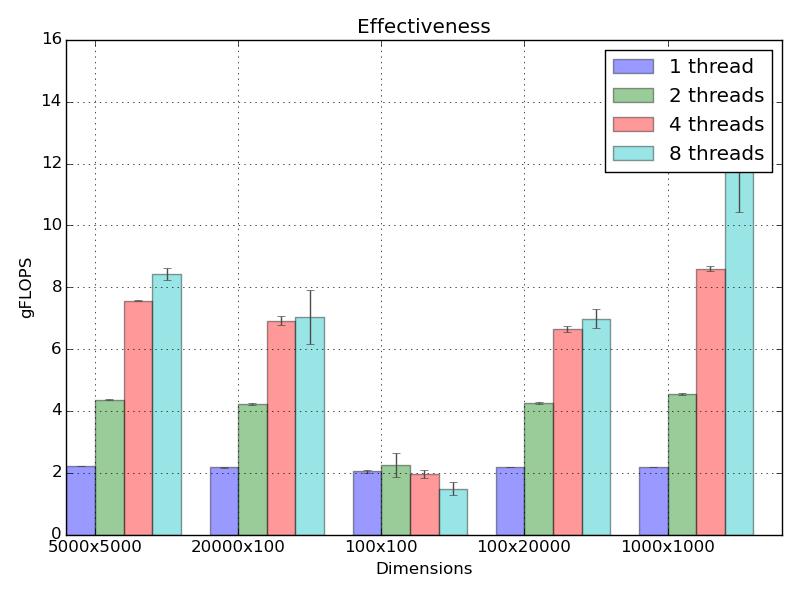
\includegraphics[width=0.75\columnwidth]{effectivness.png}

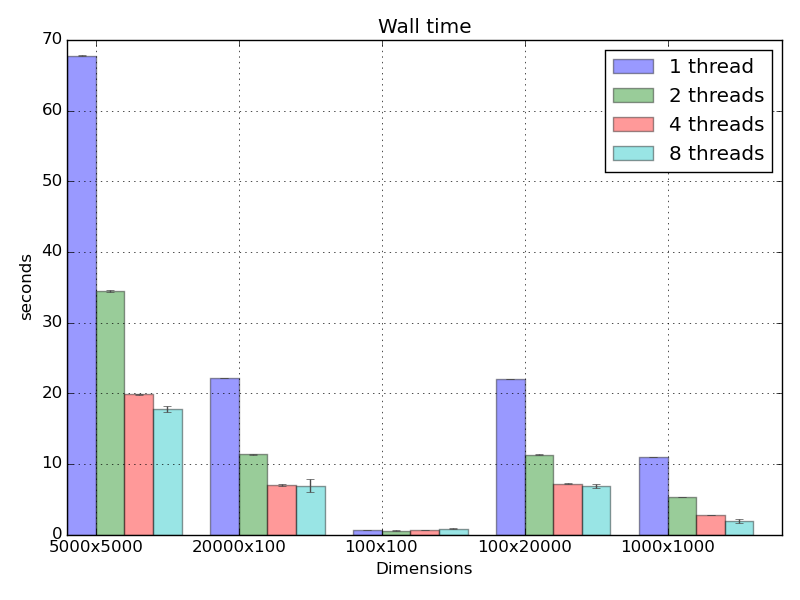
\includegraphics[width=0.75\columnwidth]{walltime.png}

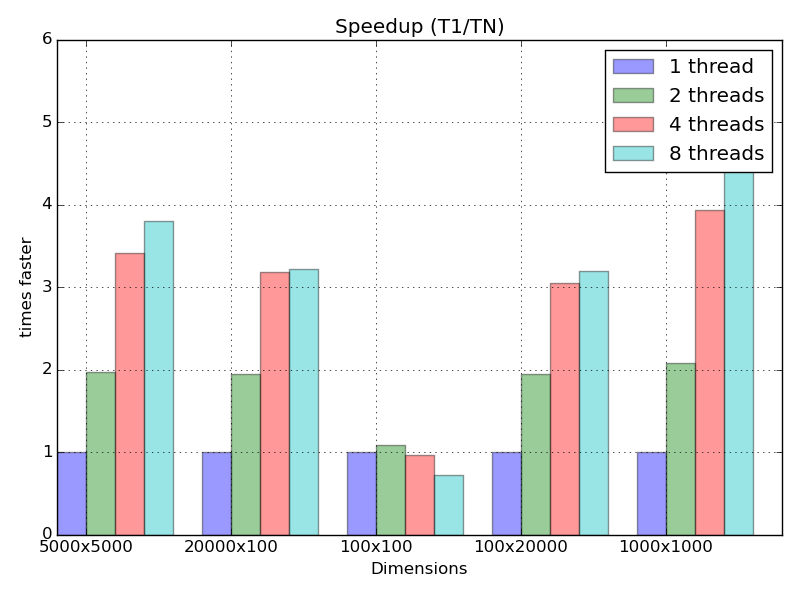
\includegraphics[width=0.75\columnwidth]{speedup.png}

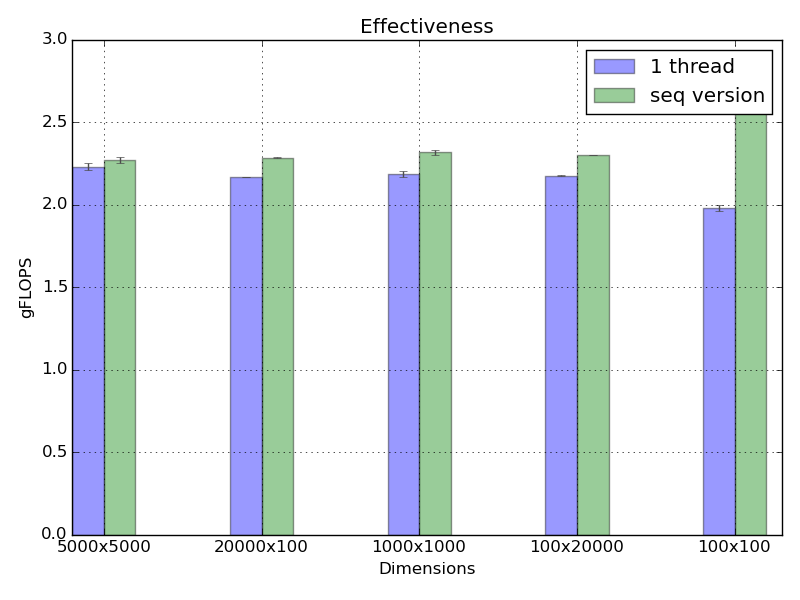
\includegraphics[width=0.75\columnwidth]{effect_seq_cmp.png}

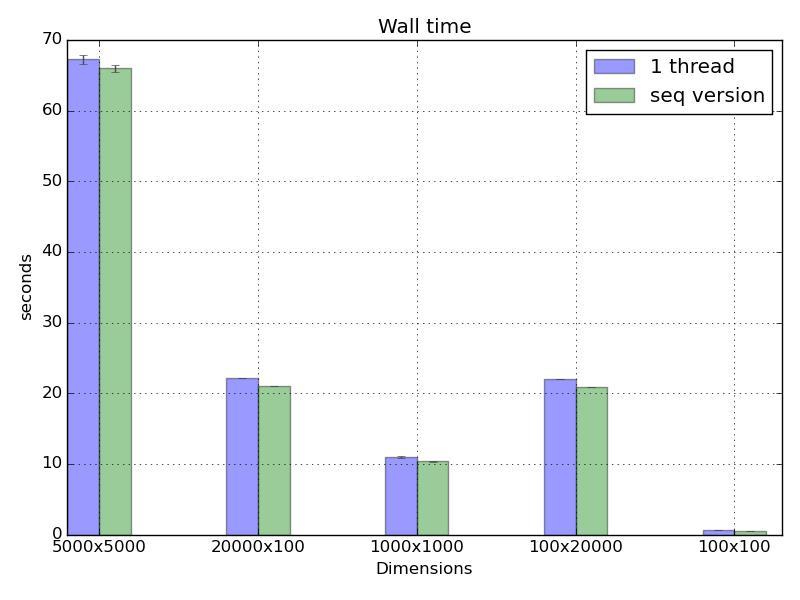
\includegraphics[width=0.75\columnwidth]{wt_seq_cmp.png}

As you can see, the results for 8 threads are extremely suspicious. We concluded that the most
likely explanation is due to the fact that we're 8 threads plus a master thread, and that since
the master thread must wake up for all threads to pass the barrier, we are presumably encountering
scheduling problems on the 8-core machines.

\textbf{Tweaks and improvements}

We made two major changes to the dissipation code after the above experiments:

\begin{enumerate}

\item Doing computation on the master thread: we only spawn $n-1$ threads (when
asked to use $n$ threads), and do the remaining computation on the master thread.
This improved the situation for 8 threads, but (as we will see) not enough.

\item Removing two barriers: we reduced the number of barriers to one single barrier,
by making threads maintain more state themselves (specifically the iteration count,
which they can all check individually to see whether they should do reduction or stop
iterating). This didn't lead to a substantial performance improvement.

\end{enumerate}

\textbf{Evaluation - Comparison with OpenMP}

As you can see from the graphs below, as mentioned already, our final performance (except in the 8-thread case
mentioned) is extremely similar to that of our previous OpenMP implementation, both without reductions
(or rather, only with a single final reduction) and with reductions at every step. This is exactly what we
expected, since the OpenMP overhead is fairly low, and we are (hopefully) doing most things in a similar
way.

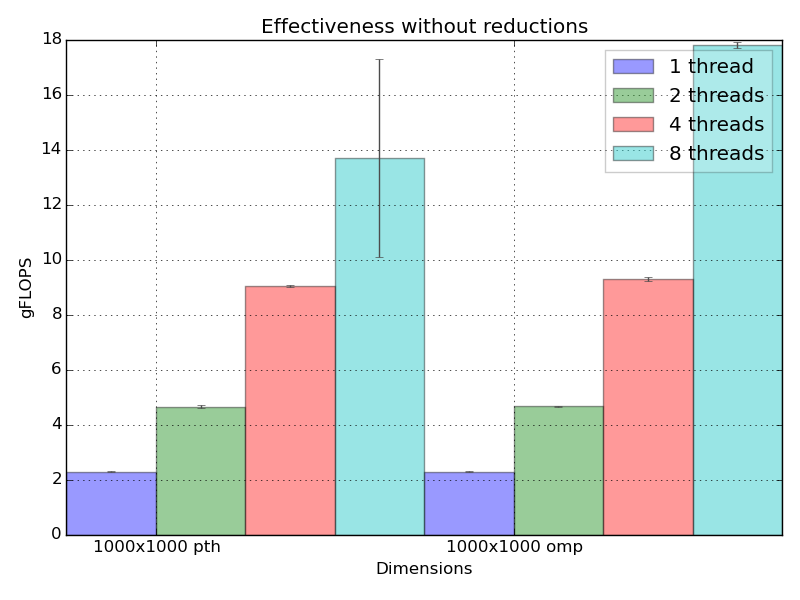
\includegraphics[width=0.75\textwidth]{pth_vs_omp_effectivness_without_reductions.png}

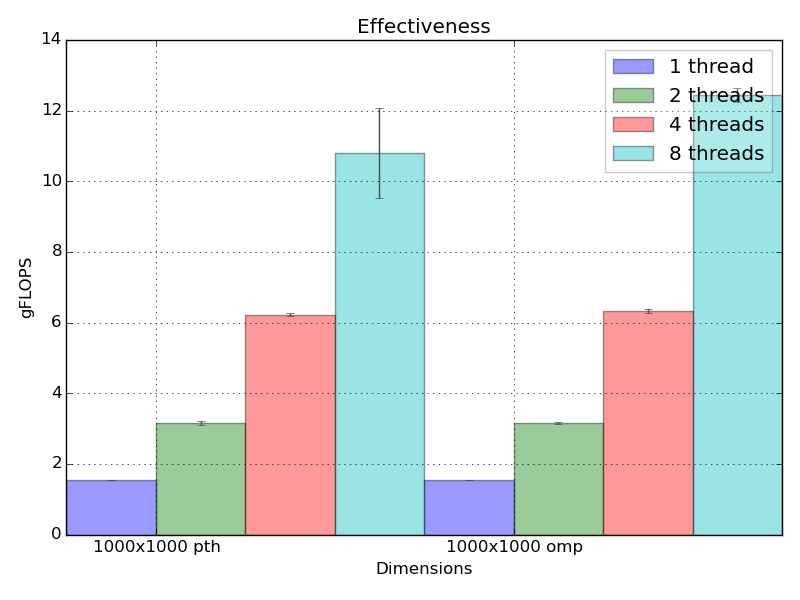
\includegraphics[width=0.75\textwidth]{pth_vs_omp_effectivness_with_reductions.png}

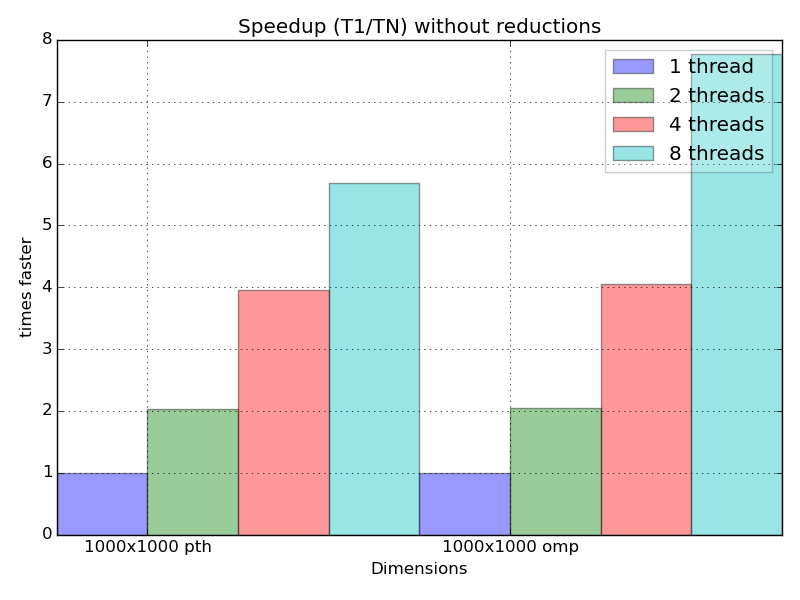
\includegraphics[width=0.75\columnwidth]{pth_vs_omp_speedup_without_reductions.png}

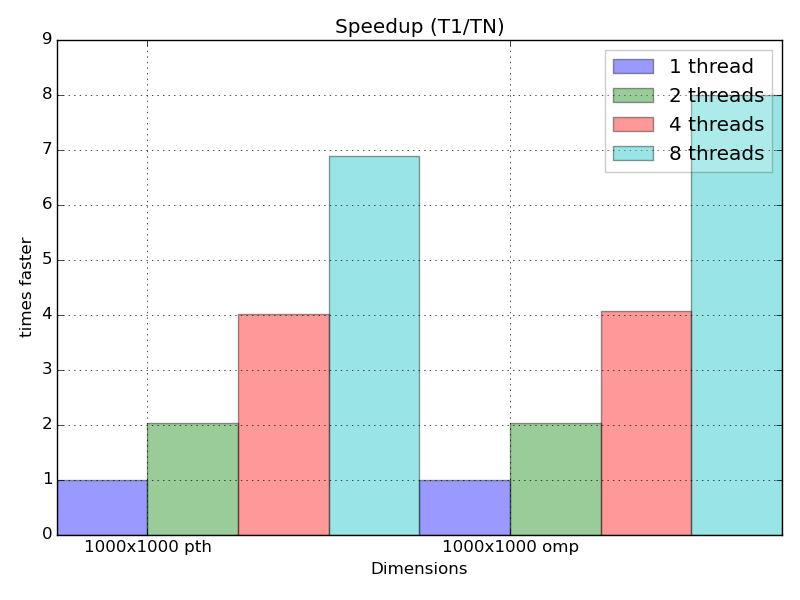
\includegraphics[width=0.75\columnwidth]{pth_vs_omp_speedup_with_reductions.png}

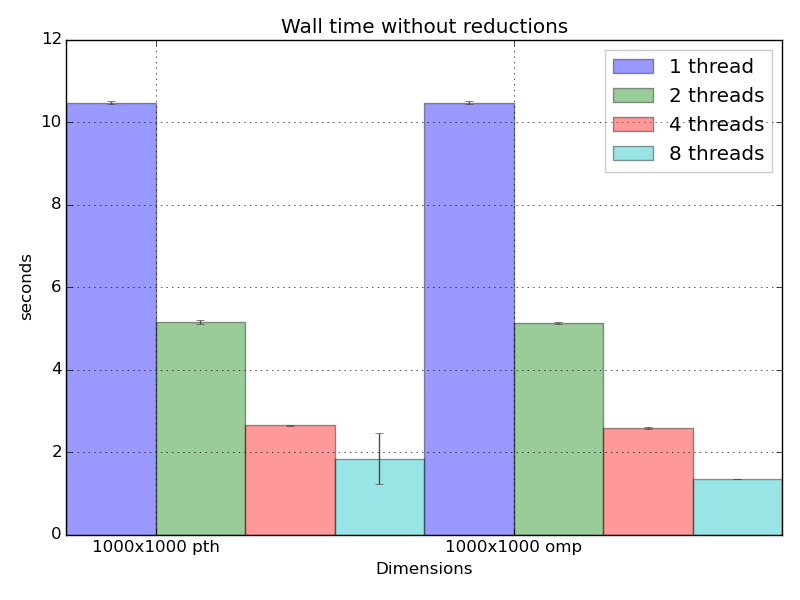
\includegraphics[width=0.75\columnwidth]{pth_vs_omp_walltime_without_reductions.png}

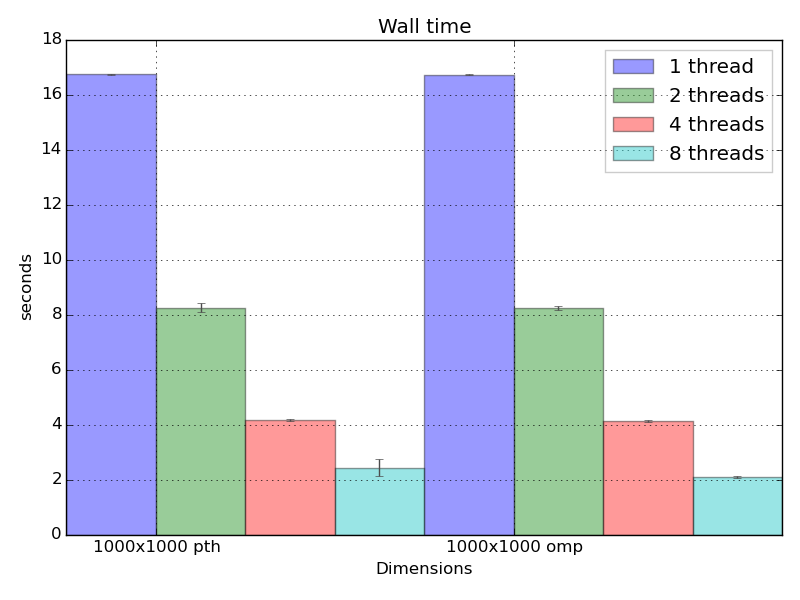
\includegraphics[width=0.75\columnwidth]{pth_vs_omp_walltime_with_reductions.png}

\textbf{Unresearched questions}

We did not explore potential improvements which could result from requesting different
behaviour from pthreads, such as pinning threads to a certain core (affinity) nor tweaking
behaviour like busywaiting.

\end{homeworkProblem}

%----------------------------------------------------------------------------------------
%	Barriers
%----------------------------------------------------------------------------------------

\begin{homeworkProblem}[Barrier synchronisation]
\textbf{Solution description}

solution desc here

\textbf{Evaluation}

experiments here

\end{homeworkProblem}

%----------------------------------------------------------------------------------------
%	Pipesort
%----------------------------------------------------------------------------------------

\begin{homeworkProblem}[Pipeline parallelism]
\textbf{Solution description}

The pipesort works as follows: The master thread creates a bounded buffer and spanws a thread associated with the buffer. After that
it generates a sequence of numbers and pushes them one by one into the buffer, thus sending them to the thread. The thread's role is 
to receive these numbers, keep the biggest value and do the same as the generator: create a new buffer plus a new thread and send the numbers
it didn't store by pushing them into the new buffer. This is done in a recursive way until the end of sequence is signaled. This occurs
by the generator sending a special symbol into the pipeline where every thread forwards it as well as its stored number to the successor. The last thread in the pipeline spawns a special thread that prints all the numbers. In the end another special symbol is forwarded which instructs the threads
to join with each other and finally end the execution. For the synchronization of the pushing and pulling from the bounded buffers we used
semaphores which are designed for this exact producer-consumer problem. Mutex locks aren't needed since for every buffer there is only a
single producer and a single consumer thus they aren't racing for particular data. Semaphores on the other hand just track the availability
of the recourses and if needed they signal blocked threads that are waiting to insert data in a full buffer or fetch data from an empty buffer.

\csnippet{sempushpull}{Semaphore handling on inserting or fetching a value}

\textbf{Evaluation}
The results are very not stable, but this is normal since a lot more threads are created than the physical cores available to handle them. This means that the scheduler plays an important role in the performance, and more importantly a role that we can't really control. In any case the following figure depicts the evaluation of the program.

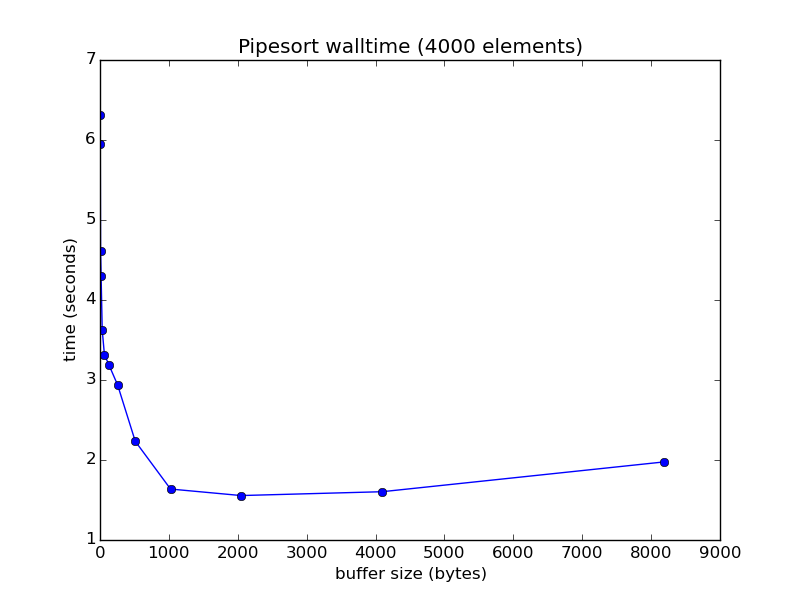
\includegraphics[width=0.75\columnwidth]{pipesort.png}

\end{homeworkProblem}

%----------------------------------------------------------------------------------------
%	critical sections
%----------------------------------------------------------------------------------------

\begin{homeworkProblem}[Mutual exclusion concepts]
\textbf{Solution description}

solution desc here

\textbf{Evaluation}

experiments here

\end{homeworkProblem}


%----------------------------------------------------------------------------------------

\end{document}
